\documentclass[aspectratio=169]{beamer}
%\documentclass{beamer}
%%%CHOOSE ASPECT RATIO ABOVE%%%

\usetheme{LU}

\usepackage[utf8]{inputenc}
\usepackage{csquotes}
\usepackage[british]{babel}
\usepackage{graphicx}
% \usepackage{booktabs}
\usepackage{makecell}
\usepackage{textcomp}

\renewcommand\theadfont{\tiny}

\title[Causal Inference]{Causal Inference in Environmental \& \newline Social Science }

\titlecolor{LUIvory} % Choose between LUPink, LULBlue, LUIvory, LUGreen
\titleimage{\includegraphics[scale=.955]{Grayscale-Globe.jpg}}
\author{Nils Droste}
\subtitle{e.g. authors}
\date{dd mm yyyy}
\institute{Lund University\\Department for Political Science}
\newcommand{\conference}{2022 ClimBEco course}

\renewcommand*{\bibfont}{\scriptsize}

% bibliography
\addbibresource{C:/Users/NILSDR~1/Dropbox/Dokumente/references/library.bib}

\begin{document}

% ------------------------------------------------------------------------------

\titleframe


% ------------------------------------------------------------------------------
% \section{Outline}

	\begin{frame}{Structure of the Course}
		\begin{table} \tiny
			\begin{tabular}{|p{1.25cm}|p{.75cm}|p{1.3cm}|p{1.3cm}|p{1.3cm}|p{1.3cm}|p{1.3cm}|}
				\hline

					& \textbf{time}
					&	\thead{ \textbf{Day 1:} \\  May 30, 2022}
					& \thead{ \textbf{Day 2:} \\  May 31, 2022}
					& \thead{ \textbf{Day 3:} \\  June 01, 2022}
					& \thead{ \textbf{Day 4:} \\  June 02, 2022}
					& \thead{ \textbf{Day 5:} \\  June 03, 2022}
					\\
				\hline
					\textbf{Lectures}
					& 10-12h
					& Greetings, \textit{Introduction to Causal inference}, and randomized controlled trials
					& \textit{(Semi) Natural Experiments}: Panel data regressions, two-way fixed effects, and recent corrections for staggered treatment
					& \textit{Simulated Counterfactuals}: matching methods, synthetic controls, and Bayesian Structural time series
					& \textit{Instruments \& Interruptions}: instrumental variables, regression discontinuity design
					& \textit{Cutting edges} : Structural equation modelling for causal inference (and machine learning techniques?)
					\\
				\hline
				 	\textbf{Seminars}
					& 13-15h
					& \textit{Replication}: Jayachandran et al. (2017) \textit{Science}
					& \textit{Replication}: Card \& Krueger (1994) \textit{JAERE}
					& \textit{Replication}: LaLonde (1986) \textit{PNAS}
					& \textit{Replication}: Abou-Chadi \& Krause (2020) \textit{RPP}
					& \textit{\textbf{Student presentations}}
					\\
				\hline
					\textbf{Consultations}
					& 15-16h
					& \thead{ \\ }
					& \thead{ \\ }
					& \thead{ \\ }
					& \thead{ \\ }
					& \thead{ \\ }
					\\
				\hline
			\end{tabular}
		\end{table}
	\end{frame}

% ------------------------------------------------------------------------------
% \section{Contract}

	\begin{frame}{Learning Contract}
		\textbf{My offer}
		\begin{itemize}
			\item I will provide you with different \textit{"entry points"} (words, graphs, math) to sharpen your intuition and conceptual understanding of quantitative causal inference
			\item We will collaboratively replicate exemplary works / causal inference strategies
		\end{itemize}
		\vspace*{.25cm}
		\textbf{My ask price}
		\begin{itemize}
			\item I want feedback what goes nice and what does not?
		\end{itemize}
		\vspace*{.25cm}
		\textbf{Your task}
		\begin{itemize}
			\item You apply one of the methods to a problem of your choice, write a short report and provide replication code
		\end{itemize}
	\end{frame}


% ------------------------------------------------------------------------------
\section{Motivation}

		% \begin{frame}{Motivation -- Question I}
		% 	\begin{center}
		% 		What examples come to mind when you think about \textit{\textbf{causality}}?
		% 	\end{center}
		% \end{frame}


	% \begin{frame}{Motivation -- Question II}
	% 	\begin{center}
	% 		Why would we even want to consider quantitative, positivist methods?
	% 	\end{center}
	% \end{frame}


		\begin{frame}{Motivation -- My answer}
			If you think about policies as if
			\vspace*{.5cm}
			\begin{itemize}
				\item they were instruments / mechanisms / interventions
				\item with a potential to fix societal problems
			\end{itemize}
			\vspace*{.5cm}
			\textit{\textbf{Would you not want to know which ones actually work?}}
		\end{frame}


		\begin{frame}{Example I: Epidemiology}
			\begin{center}
				\includegraphics[scale=.275]{Snow-cholera-map.jpg}
				\captionof{figure}{
					John Snow's original dot map of the 1854 Broad street cholera outbreak. Image sources \& info: \href{https://en.wikipedia.org/wiki/1854_Broad_Street_cholera_outbreak}{\underline{\smash{wikipedia}}}
				}
			\end{center}
			% \scriptsize\textit{"In many cases a single house has a supply different from that on either side. Each company supplies both rich and poor, both large houses and small; there is no difference in the condition or occupation of the persons receiving the water of the different companies"}
		\end{frame}



	 \begin{frame}{Motivation -- Greater minds' answers}
		\textit{Development of Western science is based on \textbf{two great achievements}: \\
		the invention of the formal logical system (in Euclidean geometry) \\
		by the Greek philosophers, and the discovery of the	possibility to find out \\ \textbf{causal relationships by systematic experiment}	(during the Renaissance).}" \\ \vspace*{.25cm}
		\textcolor{lightgray}{Albert Einstein (1953), as cited in Pearl (\citeyear{Pearl2009}), my emphasis} \\
		\vspace*{.5cm}
		\onslide<2->{
			\textit{My interpretation}: \\
			\vspace*{.25cm}
			$\rightarrow$ If we want to check our theories about how the world works, we can use systematic obervations (i.e. data) to test our assumptions. \\
			}
		\onslide<3->{
				$\rightarrow$ That does not \textit{necessarily} entail quantitative analysis, but large number of observations have benefits for robustness (see next slide).
				}
	 \end{frame}


	 	\begin{frame}{A short detour into probability}
	 		\begin{center}
	 			Is the coin fair? \\ \vspace*{.5cm}
				\only<1>{\href{https://justflipacoin.com/}{\includegraphics[scale=.15]{Flip-a-coin.png}}}
				\only<2>{\href{http://www.dataanalysisclassroom.com/lesson29/}{\includegraphics[scale=1]{cointoss.png}} \\ \vspace*{.15cm}
								 $\rightarrow$ The law of large numbers allows to aproximate "\textit{true}" values. \vspace*{.15cm}
								 % because $SE_{\overline{Y} = \frac{sd}{sqrt{n}}, larger $n$ reduce the standard error of the mean}
								}
			\end{center}
	 	\end{frame}


% ------------------------------------------------------------------------------
\section{Epistemes}

	\begin{frame}{Epistemological \& Ontological Foundations }
		\textcolor{lightgray} {BLIND MASTER PO:} \textit{Close your eyes. What do you hear?} \\ \vspace*{.1cm}
		\textcolor{lightgray} {YOUNG KWAI CHANG CAINE:} \textit{I hear the water, I hear the birds.} \\ \vspace*{.1cm}
		\textcolor{lightgray} {MASTER PO:} \textit{Do you hear your own heartbeat?} \\ \vspace*{.1cm}
		\textcolor{lightgray} {KWAI CHANG CAINE:} \textit{No.} \\ \vspace*{.05cm}
		\textcolor{lightgray} {MASTER PO:} \textit{Do you hear the grasshopper that is at your feet?} \\ \vspace*{.1cm}
		\textcolor{lightgray} {KWAI CHANG CAINE:} \textit{Old man, how is it that you hear these things?} \\ \vspace*{.1cm}
		\textcolor{lightgray} {MASTER PO:} \textit{Young man, \textbf{how is it that you do not?}} \\ \vspace*{.25cm}
		\textcolor{lightgray} {\footnotesize \textit{Kung Fu}, Pilot. Cited from \cite[(p. xi)]{Angrist2015}, own emphasis} \\ \vspace*{.5cm}

		\onslide<2->{\large {$\rightarrow$ We assume a measurable reality (\underline{\smash{\href{https://en.wikipedia.org/wiki/Positivism}{positivism}}}, \underline{\smash{\href{https://en.wikipedia.org/wiki/Empiricism}{empiricism}}}}).}
	\end{frame}


	\begin{frame}{Epistemological \& Ontological Foundations }
		 \onslide<1->{
			To answer questions of causality we need an \textit{epistemological framework} to
			\vspace*{.25cm}
			\begin{itemize}
				\item formulate testable hypothesis
				\item find a suitable method to test hypothesis
			\end{itemize}
			\vspace*{.5cm}
		}
		\onslide<2->{
			Statistical causal inference is \textit{one} such approach, suitable for
			\vspace*{.25cm}
			\begin{itemize}
				\item both inductive and deductive reasoning
				\item generalizable, reproducible, falsifiable research
			\end{itemize}
		}
	\end{frame}

% ------------------------------------------------------------------------------

\section{Causation}

	\begin{frame}{Causation}
		We have a population of units; for each unit $i$ we observe a variable $D$ and a variable $Y$. \\
		\vspace*{.5cm}
		\onslide<2->{We observe that $D$ and $Y$ are correlated. Does \textit{correlation} imply \textit{causation}? \\
		\vspace*{.5cm}}
		\onslide<3->{
			\textbf{In general no}, because of \\
			\begin{itemize}
				\item confounding factors;
				\item reverse causality
			\end{itemize}
			\vspace*{.5cm}
		}
		\onslide<4->{
			We would like to understand in which circumstances one can conclude from the evidence that {D causes Y}. \\
			\vspace*{.5cm}
			\textcolor{lightgray} {\footnotesize{source: lecture notes Sascha Becker 2014}}
		}
	\end{frame}


	\begin{frame}{Example II:  Storcks \& Babies }
		\begin{center}
		\includegraphics[scale=1.125]{Storcks.png}
		\captionof{figure}{
				Do storcks deliver babies? Image source: Matthews (\citeyear{Matthews2000})
			}
		\end{center}
	\end{frame}


	\begin{frame}{Example II:  Storcks \& Babies }
		What happened, why did we get it so wrong?
		\begin{center}
		\includegraphics[scale=.18]{Babies.png}
		\captionof{figure}{
				Subset of original data. Source: Matthews (\citeyear{Matthews2000})
			}
		\end{center}
		\footnotesize{Besides \textcolor{red}{outcome variable} and \textcolor{blue}{variable of interest}, we forgot \textcolor{green}{confounding variables}.}
		\begin{equation}
			\textcolor{red}{Y}_i = \alpha + \beta_1 \textcolor{blue}{D}_i + \beta_2 \textcolor{green}{C}_i + \varepsilon_i
		\end{equation}
	\end{frame}


	\begin{frame}{Problem I: Confounding variables}
		\begin{columns}
			\begin{column}{0.5\textwidth}
				\begin{center}
				\includegraphics[scale=.5]{dag-control.png}
				\captionof{figure}{
						Directed acyclic graph where variable \textcolor{green}{C} affects both textcolor{blue}{D} and \textcolor{red}{Y}. Image source: Modified from \href{http://nickchk.com/causalgraphs.html}{\underline{\smash{Huntington-Klein 2018}}}
					}
				\end{center}
			\end{column}
			\begin{column}{0.5\textwidth}  %%<--- here
			    \begin{center}
			     \animategraphics[width=\textwidth,controls]{10}{AnimationofControl-}{0}{199}
			    \end{center}
			\end{column}
		\end{columns}
	\end{frame}

% ------------------------------------------------------------------------------

\section{Theory}

	\subsection{Neyman-Rubin Model}

		\begin{frame}{Neyman-Rubin Model I}
			Recall, we let $\textcolor{red}{Y}$ denote our outcome variable, and $\textcolor{blue}{D}$ our treatment or intervention which we are interested in. \\ \vspace*{.25cm}
			Letter $i$ is an index of the individuals within our population. \\
			\vspace*{.25cm}
			\onslide<2->{For $\textcolor{blue}{D}$ we have two possible realizations:}
			\onslide<3->{
				\vspace*{.25cm}
				\begin{itemize}
					\item $\textcolor{blue}{D}=\textcolor{blue}{1}$ if $i$ has received treatment;
					\item $\textcolor{blue}{D}=\textcolor{blue}{0}$ if $i$ has \textit{not} received treatment.
				\end{itemize}
			}
			\onslide<4->{
				\vspace*{.125cm}
				Thus, $\textcolor{red}{Y}_i(\textcolor{blue}{D}_i)$ indicates the \textit{potential outcome} according to treatment:
				\vspace*{.125cm}
				\begin{itemize}
					\item $\textcolor{red}{Y}_i(\textcolor{blue}{1})$ is the outcome in case of treatment;
					\item $\textcolor{red}{Y}_i(\textcolor{blue}{0})$ is the outcome in case of \textit{no} treatment.
				\end{itemize}
			}
		\end{frame}


		\begin{frame}{Neyman-Rubin Model II}
			The hypothetical outcome for each unit can be written as
			\begin{equation}
				\Delta \textcolor{red}{Y}_i = \textcolor{red}{Y}_i(\textcolor{blue}{1}) - \textcolor{red}{Y}_i(\textcolor{blue}{0}) % \text{, or alternatively} = (\textcolor{red}{Y}_i|1) - (\textcolor{red}{Y}_i|0)
			\end{equation}
			\begin{itemize}
				\item<2-> This approach requires to think in terms of “\textit{counterfactuals}”. \\ \vspace*{.125cm}
				\item<3-> While theoretically ideal, the identification and the measurement of a pure counterfactual is logically impossible: \\ \vspace*{.125cm}
				\item<4-> We can only observe one state of the world, i.e. we cannot \textit{directly} measure what would have happened in the counterfactual case (cf. \cite{Holland1986}).
			\end{itemize}
		\end{frame}


		\begin{frame}{Neyman-Rubin Model III}
			\onslide<1->{The best we can do to infer an average treatment effect (ATE) by comparing sufficiently large subsamples from the overall population $I$: i.e. $ I =\{A,B...\} $. \\
			\vspace*{.125cm}}
			\onslide<2->{Say, we expect the outcome to be
			\begin{equation}
				E \{\Delta \textcolor{red}{Y}_i \} = E \{\textcolor{red}{Y}_i(\textcolor{blue}{1}) - \textcolor{red}{Y}_i(\textcolor{blue}{0}) \} = E \{\textcolor{red}{Y}_i(\textcolor{blue}{1}) \} - E \{\textcolor{red}{Y}_i(\textcolor{blue}{0}) \}.
			\end{equation} \\ }
			\onslide<3->{We can approximate this theoretical effect by treating individuals $a$ from $A$, and compare their average to the one of untreated individuals $b \in B$: \\
			\begin{equation}
				E \{\Delta \textcolor{red}{Y}_i \}  \approx  E \{\textcolor{red}{Y}_a(\textcolor{blue}{1})\} - E \{\textcolor{red}{Y}_b(\textcolor{blue}{0})\}
			\end{equation} \\ }
			\onslide<4->{In this case we exploit \textit{random chance} within sufficiently large samples that makes these groups comparable. Such a setting can be generated by randomized controlled experiments.}
		\end{frame}


	\subsection{Structural Causal Models}

		\begin{frame}{Structural Causal Models I}
			Another approach is to specify the assumed causal relation within a system by directed acyclic graphs (DAG).
			For example:
			\vspace*{.125cm}
			\begin{columns}
				\begin{column}{0.5\textwidth}
					\onslide<1->{
						\begin{center}
						\includegraphics[scale=.5]{dag_basic.png}
						\vspace*{.925cm}
						\captionof{figure}{
								Directed acyclic graph where D affects Y. Image source: modified from \href{http://nickchk.com/causalgraphs.html}{\underline{\smash{Huntington-Klein 2018}}}
							}
						\end{center}
					}
				\end{column}
				\begin{column}{0.5\textwidth}
					\onslide<2->{
						\begin{center}
						\includegraphics[scale=.5]{dag_extended.png}
						\captionof{figure}{
								Directed acyclic graph where variable C affects both D and Y. Image source: \href{http://nickchk.com/causalgraphs.html}{\underline{\smash{Huntington-Klein 2018}}}
							}
						\end{center}
					}
				\end{column}
			\end{columns}
			\onslide<3->{\vspace*{.125cm} In the second case we need to close the \href{https://stats.stackexchange.com/questions/350267/a-layman-understanding-of-the-difference-between-back-door-and-front-door-adjust}{\underline{\smash{\textit{back-door path}}}} by controlling for $\textcolor{green}{C}$.}
		\end{frame}


		\begin{frame}{Structural Causal Models II}
			Judea Pearl et al. (\cite*{Pearl2016}) developed the do-calculus to express the effect of an intervention you \textit{do}: \\ \vspace*{.125cm}

			\onslide<2->{$P(\textcolor{red}{Y}|\textcolor{blue}{D})$ is the \textit{conditional probability} of $\textcolor{red}{Y}$ given $\textcolor{blue}{D}$. \\ \vspace*{.125cm}}

			\onslide<3->{If we have a confounding variable $\textcolor{green}{C}$ and we want an unbiased estimate of intervention $\textcolor{blue}{D}$'s effects on $\textcolor{red}{Y}$, we shall control for $\textcolor{green}{C}$ and assess the probability of $\textcolor{red}{Y}$ given both $\textcolor{blue}{D}$ and $\textcolor{green}{C}$:}

			\onslide<4->{
				\begin{equation}
					P(\textcolor{red}{Y}|do(\textcolor{blue}{D})) = \sum_{\textcolor{green}{C}} P(\textcolor{red}{Y}|\textcolor{blue}{D},\textcolor{green}{C})P(\textcolor{green}{C})
				\end{equation}
			}
		\end{frame}


	\subsection{Mechanism}

		\begin{frame}{Mechanism}
			Specifying a model is a necessary but not a sufficient condition to understand causality. Our model also needs to resemble reality. \\ \vspace*{.25cm}
			\onslide<2->{We therefore need an understanding of the underlying \textit{\textbf{mechanism}}. \\ \vspace*{.25cm}}
			\onslide<3->{
				\begin{center}
					\textit{“Causal processes, causal interactions, and causal laws provide the mechanisms by which the world works; to understand why certain things happen, we need to see how they are produced by these mechanisms.”}
					\\ \vspace*{.1cm}
					\scriptsize{\textcolor{gray}{\cite{Salmon1984} as cited in \underline{\smash{\href{http://www.skleinberg.org/teaching/CI18/index.html}{Samantha Kleinberg}}} \underline{\smash{\href{http://www.skleinberg.org/teaching/CI18/lecture9.pdfl}{Causal Inference, lecture 9}}}} \\ \vspace*{.25cm}}
				\end{center}
			}
			\onslide<4>{My take: $\rightarrow$ \textit{\textbf{We need theory!}} Theory can be developed (and tested) through many (inductive \& deductive) methods.}
		\end{frame}

		\begin{frame}{Ontology - Epistemology - Theory}
			\begin{center}
					\includegraphics[scale=.1625]{PlatosCave.jpg}
					\captionof{figure}{
						Plato's allegory of the cave. Image source: \href{https://s.studiobinder.com/wp-content/uploads/2019/12/Platos-Allegory-of-the-Cave-Featured-Image-1.jpg}{\underline{\smash{Studio Binder 2020}}}
				}
			\end{center}
		\end{frame}

% ------------------------------------------------------------------------------
%
% \section{Probability Puzzle}
% 	\begin{frame}{The Monty Hall Problem I}
% 		\begin{center}
% 			\includegraphics[scale=1]{MontyHall.png}
% 			\captionof{figure}{The (in)famous Monty Hall Problem. Image source: \href{https://en.wikipedia.org/wiki/Monty_Hall_problem}{\underline{\smash{wikipedia}}}}
% 		\end{center}
% 	\end{frame}
%
% 	\begin{frame}{The Monty Hall Problem II: solution}
% 		\begin{center}
% 			\includegraphics[scale=.6]{MontyHall2.png}
% 			\captionof{figure}{Solving the Monty Hall problem (cf. \cite{Selvin1975a, Selvin1975b}). Image source: \href{https://en.wikipedia.org/wiki/Monty_Hall_problem}{\underline{\smash{wikipedia}}}}
% 		\end{center}
% 	\end{frame}

% ------------------------------------------------------------------------------
% \section{Intermediate Learning Outcomes}

	\begin{frame}{Intermediate lessons}
		Do you have developed an intuition for the following?
		\vspace*{.5cm}
		\onslide<2->{
			\begin{itemize}
				\item<2-> How large numbers of obervations allow more robust inference?
				\item<3-> That correlation does not imply causation?
				\item<4-> That causal analysis require some form of framework to {...}
				\begin{itemize}
					 \item formulate hypothesis
					 \item test hypothesis ?
				\end{itemize}
				\item<5-> That quantitative causal inference needs theory / an understanding of the causal mechanism to work?
			\end{itemize}
		}
	\end{frame}

% ------------------------------------------------------------------------------
\section{Controlled Trials}
	\begin{frame}{The history of randomized controlled trials (RCT)}
		\begin{itemize}
			\item<2-> \textcolor<3->{gray}{1747 James Lind conducted a clinical trial on the treatment of scurvy}
			\item<3-> \textcolor<4->{gray}{19th century: experimental psychology (Wilhelm Wundt)}
			\item<4-> \textcolor<5->{gray}{up to early 20th century: experimental sociology (Comte vs. Hegel vs. Marx)}
			\item<5-> \textcolor<6->{gray}{Ronald Fisher's 1935 \textit{Design of Experiments} (agricultural field experiments)}
			\item<6-> \textcolor<7->{gray}{since 1960's standard for approval of medicine (double blind clinical trials)}
			\item<7-> \textcolor<8->{gray}{1970's RAND Health Insurance Experiment (cf. \cite{Angrist2015})}
			\item<8-> \textcolor<9->{gray}{2019 Nobel Prize in Economics to \textit{randomistas} (\cite{Banerjee2011})}
		\end{itemize}
		\vspace*{.25cm}
		 \onslide<9->{\textcolor{gray}{References and further reading}
			\begin{itemize}
				\item \textcolor{gray}{RCTs: \cite{Pearce2014, DeSouzaLeao2019, Jamison2019}}
				\item \textcolor{gray}{Experiments in a broader sense, cf. \href{https://en.wikipedia.org/wiki/Timeline_of_scientific_experiments}{\underline{\smash{Wikipedia}}},
				\href{https://www.britannica.com/topic/Western-philosophy/Analytic-philosophy}{\underline{\smash{Britannica}}}
				}
			\end{itemize}
			}
	\end{frame}

% ------------------------------------------------------------------------------
\section{Design}
	\begin{frame}{Experiments -- the "gold" standard}
		In order to assess the effect of a "treatment" (of sorts), we can \\ \vspace*{.125cm}
		\begin{itemize}
			\item<2-> take two random samples from a population
			\item<3-> treat one, and compare it to the other (as if "counterfactual")
		\end{itemize}
		\vspace*{.125cm}
		\onslide<4->{
		\begin{center}
			\includegraphics[scale=.15]{RCT.jpg}
			\captionof{figure}{Schematic outline of a randomized controlled trial. Image source: Adapted from \cite{Kendall2003}}
		\end{center}}
	\end{frame}

	\begin{frame}{Experiments -- statistical approach}
		\onslide<1->{Recall that we approach the average treatment effect (ATE) by comparing sufficiently large subsamples from the overall population: i.e. $ I =\{A,B...\} $. \\
		\vspace*{.25cm}}
		\onslide<2->{To approximate this treatment effect we can treat individuals $a \in A$, and compare their average to the one of untreated individuals $b \in B$. \\ This is called a \textit{difference-in-means} estimator: \\
		\begin{equation}
			E \{\Delta \textcolor{red}{Y}_i \}  \approx  E \{\textcolor{red}{Y}_a(\textcolor{blue}{1})\} - E \{\textcolor{red}{Y}_b(\textcolor{blue}{0})\}
		\end{equation} \\ \vspace*{.25cm} }
		\onslide<3->{\textit{Random chance} in sufficiently large samples makes these groups comparable (remember the law of large numbers).}
	\end{frame}

	\begin{frame}{Experiments -- graphical approach}
		\begin{center}
			\includegraphics[scale=.33]{Caffeine.jpg}
			\captionof{figure}{A hypothetical experiment. Image source: Adapted from \href{http://personality-project.org/r/basics.t.html}{\underline{\smash{personality-project}}}}
		\end{center}
	\end{frame}

	\begin{frame}{Experiments -- methodological note of caution}
		When designing an experiment we need a \textbf{big enough sample size}. \\ \vspace*{.25cm}
		What is big enough can be calculated based on \\ \vspace*{.25cm}
		\begin{itemize}
			\item false positive probability (e.g. no more than 5\%)
			\item minimum detectable effect (MDE)
			\item the power required at MDE (e.g. 80\%)
		\end{itemize}
		\vspace*{.5cm}
		\scriptsize{\textcolor{gray}{Reference: cf. \cite{Coleman2018} or \underline{\smash{\href{http://web.stanford.edu/~rjohari/teaching/notes.html}{Ramesh Johari}}} \underline{\smash{\href{http://web.stanford.edu/~rjohari/teaching/notes/226_lecture18_causal.pdf}{MS\&E 226 lecture 18}}}}}
	\end{frame}

% ------------------------------------------------------------------------------
\section{Empirics}
	\subsection{Conservation}
		\begin{frame}{Paying households for conservation}
			\begin{center}
				\includegraphics[scale=.4]{CashforCarbon.jpg}
			\end{center}
		\end{frame}

		\begin{frame}{Paying households for conservation}
			\textcolor<2->{gray}{Deforestation contributes to climate change.\\ \vspace*{.25cm}}
			\begin{itemize}
				\item<2-> \textcolor<3->{gray}{As much land is private, paying land users for conservation (a public good) is a common approach.}
				\item<3-> \textcolor<4->{gray}{Payments for ecosystem services (PES) schemes became popular (in the developing world).}
				\item<4-> \textcolor<5->{gray}{Jayachandran et al. (\cite*{Jayachandran2017}) run an experiment in Uganda (third highest deforestation rate in the world 2005-2010)}
				\item<5-> \textcolor<6->{gray}{They}
				\begin{itemize}
					\item \textcolor<6->{gray}{pay 563 private forest owners (PFO) in 60 treated villages (there are 535 PFO in 61 control villages), and}
					\item \textcolor<6->{gray}{monitor deforestation rates by satelite imagery.}
				\end{itemize}
				\item<6-> Jayachandran et al. (\cite*{Jayachandran2017}) analyse the effect on tree cover.
			\end{itemize}
		\end{frame}

		\begin{frame}{Paying households for conservation}
			\textbf{Results} \\
			\only<1-2>{
					\only<1>{\vspace*{.26cm} Primary outcomes \\ \begin{center} \vspace*{.22cm} \includegraphics[scale=.66]{CashforCarbon_Results_1.png} \vspace*{.15cm} \end{center}}
					\only<2>{\vspace*{.25cm} Secondary outcomes \\ \begin{center} \vspace*{.25cm} \includegraphics[scale=.66]{CashforCarbon_Results_2.png} \end{center}}
				}
			\onslide<3->{
				\vspace*{.44cm}
				\onslide<3-> \textcolor<5->{gray} {Paying forest owners for conservation reduces deforestation rates \\ $\rightarrow$ No afforestation is observable at that payment level. \\ \vspace*{.5cm}}
				\onslide<4-> \textcolor<5->{gray} {"This study also adds to the literature on PES [by]"} \\ \vspace*{.25cm}
				\begin{itemize}
					\item<4-> \textcolor<5->{gray} {"satellite images with very high resolution, which enables us to detect selective tree-cutting in addition to clear-cutting"}
					\item<5-> "cost-benefit analysis allows policy-makers to assess the cost-effectiveness of the PES program in comparison to other options for reducing global carbon emissions"
				\end{itemize}
				\vspace*{.5cm}
				}
			\textcolor{gray}{\scriptsize{\cite[p. 6]{Jayachandran2017}}}
		\end{frame}

	\begin{frame}{Paying households for conservation}
		\textbf{A note on methods} \\ \vspace*{.5cm}
		The authors used a \textit{stratification} strategy to ensure balanced randomization: \\ \vspace*{.5cm}
		\begin{columns}
			\begin{column}{0.5\textwidth}
				\begin{itemize}[<+->]
					\item number of PFOs
					\item av. household earnings / capita
					\item distance to a road, and
					\item average landsize
				\end{itemize}
				\vspace*{1cm}
			\end{column}
			\begin{column}{0.5\textwidth}
				\begin{center}
					\includegraphics[scale=.25]{Stratified_sampling.png}
					\captionof{figure}{\textcolor{gray}{Image source: \href{https://en.wikipedia.org/wiki/Stratified_samplingl}{\underline{\smash{wikipedia}}}}}
				\end{center}
			\end{column}
		\end{columns}
	\end{frame}

	\begin{frame}{Paying households for conservation}
		\textbf{Discussion questions} \\ \vspace*{.25cm}
		\begin{itemize}
			\item Do you think it is a good idea to pay private land owners for the provision of public goods \/ ecosystem services?
			\item Do you think it is a market-based approach if the government pays it? If so why?
			\item What could be alternative approaches to ensure provision of public (environmental) goods?
		\end{itemize}
	\end{frame}

% ------------------------------------------------------------------------------
\section{Randomistas}
	\begin{frame}{Randomistas on a roll}
		\only<1>{Increased use of development policy evaluation studies (or RCTs)
			\begin{center}
			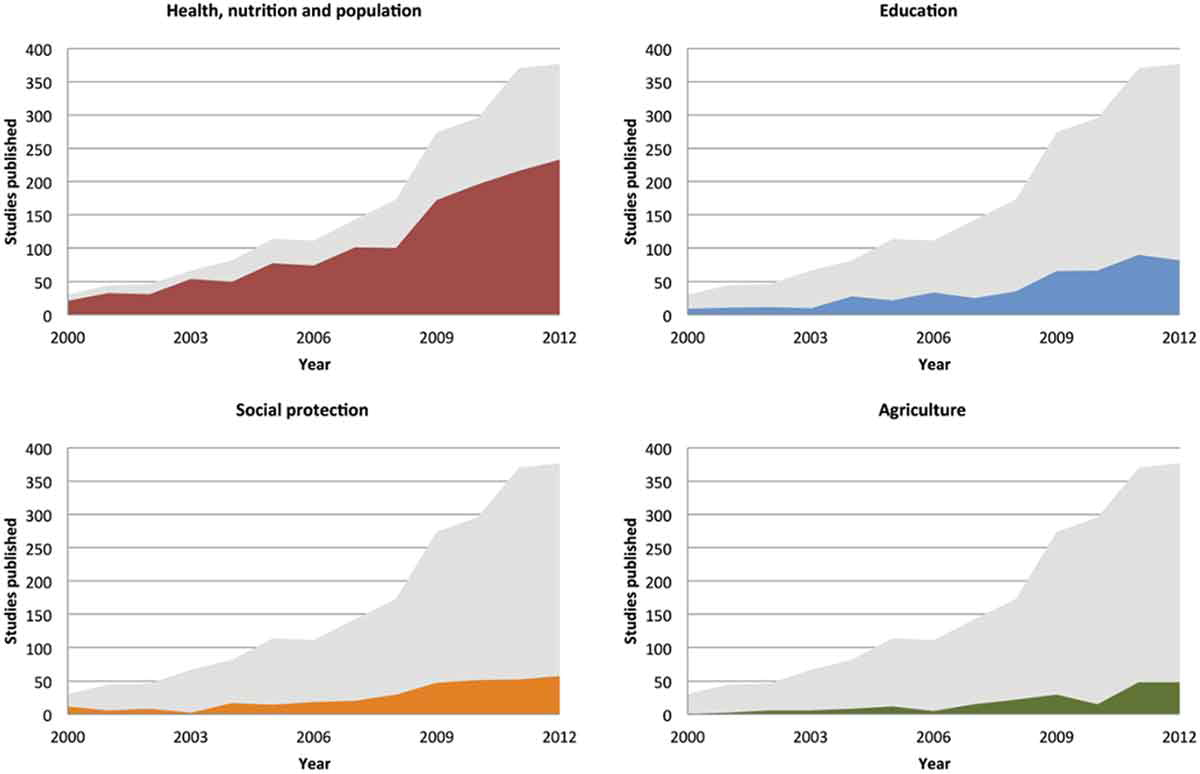
\includegraphics[scale=.2]{ImpactEvaluation.jpeg}
			\captionof{figure}{\textcolor{gray}{Share of quasi-experimental studies in color. Image source: Cameron et al. \cite*{Cameron2016}, cf. \cite{Tollefson2015}}}
			\end{center}
			}
		\only<2>{
			\begin{center}
			\includegraphics[scale=.3]{NobelPrize.jpg}
			\captionof{figure}{\textcolor{gray}{Banerjee, Duflo \& Kremer win the 2019 Nobel Prize in Economics. \\
			Image source: \href{https://www.nobelprize.org/prizes/economic-sciences/2019/summary/}{\underline{\smash{Sverige Riksbank}}}}}
			\end{center}
			}
	\end{frame}

% ------------------------------------------------------------------------------
% \section{Critical Voices}
	\begin{frame}{Not all that glitters is gold}
		\begin{itemize}[<+->]
			\item \textcolor<2->{gray}{Some treatments cause ethical concern.}
			\item \textcolor<3->{gray}{RCTs target individuals not structural causes.}
			\item \textcolor<4->{gray}{A solid design is needed for internal and external validity.}
			\item \textcolor<5->{gray}{There is / was a replication crisis and p-hacking.}
			\item \textcolor<6->{gray}{There can be secondary, unintended outcomes.}
			\item Experiments can be costly.
		\end{itemize}
	\end{frame}

	\begin{frame}{A rejoinder}
	 	\begin{itemize}[<+->]
			\item \textcolor<2->{gray}{Experiments do not deliver all answers (cf. \cite{Howe2004})}
			\item \textcolor<3->{gray}{A fuller picture may be provided by mixed method research \\ (cf. \cite{Imai2011,Latour2012,Blok2014})}
			\item Observational data and identification strategies provide alternative quantitative approaches for causal inference (cf. \cite{Gelman2014})
	 	\end{itemize}
	 	\vspace*{.5cm}
		 	\onslide<4>{$\rightarrow$ \textit{My own take}: I believe more systematical experiments in the implementation of policies can increase effectiveness (compared to trial-and-error)}
	\end{frame}

% ------------------------------------------------------------------------------
% \section{Learning Outcomes}
	\begin{frame}{Econometricians}
		\footnotesize{
		\textcolor{lightgray} {MASTER JOSHWAY:} \textit{In a nutshell, please, Grasshopper.} \\ \vspace*{.1cm}
		\textcolor{lightgray} {GRASSHOPPER:} \textit{Causal inference compares potential outcomes, descriptions of the world when alternative roads are taken.} \\ \vspace*{.1cm}
		\textcolor{lightgray} {MASTER JOSHWAY:} \textit{Do we compare those who took one road with those who took another?} \\ \vspace*{.1cm}
		\textcolor{lightgray} {GRASSHOPPER:} \textit{Such comparisons are often contaminated by selection bias, that is, differences between treated and control subjects that exist even in the absence of a treatment effect.} \\ \vspace*{.1cm}
		\textcolor{lightgray} {MASTER JOSHWAY:} \textit{Can selection bias be eliminated?} \\ \vspace*{.1cm}
		\textcolor{lightgray} {GRASSHOPPER:} \textit{Random assignment to treatment and control conditions eliminates selection bias. Yet even in randomized trials, we check for balance.} \\ \vspace*{.1cm}
		\textcolor{lightgray} {MASTER JOSHWAY:} \textit{Is there a \textbf{single causal truth}, which all randomized investigations are sure to reveal?} \\ \vspace*{.1cm}
		\textcolor{lightgray} {GRASSHOPPER:} \textit{I see now that there can be \textbf{many truths}, Master, some compatible, some in contradiction. We therefore take special note when findings from two or more experiments are similar.} \\ \vspace*{.2cm}}
		\textcolor{lightgray} {\scriptsize{\cite[(p. 30)]{Angrist2015}, own emphasis}}
	\end{frame}

	\begin{frame}{Experiment lessons}
		\begin{itemize}
			\item The design of the experiments matter for it's
			\begin{itemize}
				 \item (internal and external) validity
				 \item ethical implications
			\end{itemize}
			\item Interpretation of the results is a big part of the story / political recommendation.
		\end{itemize}
	\end{frame}
% ------------------------------------------------------------------------------
% \section{Further readings}
	\begin{frame}{Further readings}
		\footnotesize
		\begin{itemize}
			\item Behaghel, L., Macours, K., \& Subervie, J. (2019). How can randomised controlled trials help improve the design of the common agricultural policy?  \textit{European Review of Agricultural Economics}, 46(3), 473-493. doi: \href{https://doi.org/10.1093/erae/jbz021}{10.1093/erae/jbz021}
			\item Beaman, L., Duflo, E., Pande, R., \& Topalova, P. (2012). Female leadership raises aspirations and educational attainment for girls: A policy experiment in India. \textit{Science, 335}(6068), 582-586. doi: \href{https://doi.org/10.1126/science.1212382}{10.1126/science.1212382}
			\item Braga, A. A., \& Bond, B. J. (2008). Policing crime and disorder hot spots: A randomized controlled trial.  \textit{Criminology}, 46(3), 577-607. doi: \href{https://doi.org/10.1111/j.1745-9125.2008.00124.x}{10.1111/j.1745-9125.2008.00124.x}
		\end{itemize}
	\end{frame}

% ------------------------------------------------------------------------------
	\begin{frame}[t, allowframebreaks]{References}
	% [t,allowframebreaks]
	  \printbibliography
	\end{frame}
% ------------------------------------------------------------------------------

%
\end{document}
